\section{Buck-, Boost- und Buck-Boost-Converter}
DC-DC-Wandler sind spezielle Gleichstromsteller
Diese Section behandelt die wichtigsten nichtisolierten Gleichstromsteller zur
Spannungsanpassung in DC-Systemen.  
Sie unterscheiden sich von den klassischen Gleichstromstellern durch ihre
spezifische Topologie und ihren kontinuierlichen Energietransfer über eine Induktivität.

\smallskip
\paragraph{Grenzinduktivität für kontinuierlichen Betrieb}
\[
L_{\min} = \frac{(1-d)R}{2 f_s}
\]


\textbf{Zielbild:}
\begin{itemize}
    \item Grundprinzip der drei wichtigsten DC-DC-Wandler verstehen
    \item Mittelwertzusammenhänge kennen
    \item Einordnung zu Gleichstromstellern beherrschen
\end{itemize}

% -------------------------------------------------
\subsection{Allgemeines Grundprinzip}

Alle DC-DC-Wandler arbeiten mit:

\begin{itemize}
    \item Schalter
    \item Diode (oder synchroner Schalter)
    \item Induktivität $L$
    \item Glättkondensator $C$
\end{itemize}

Grundgleichung (idealer Fall, stationär):

\[
\cbl{u_L = L \frac{di_L}{dt}}
\qquad
\Rightarrow
\qquad
\cbl{\overline{u_L} = 0}
\]

\crd{\textrightarrow\ Im stationären Zustand ist der Mittelwert der Induktionsspannung null.}

% -------------------------------------------------
\subsection{Buck-Converter (Abwärtssteller)}

% --- HIER: bestehende oder spätere Grafik Buck ---
Buck-Converter (Abwärtssteller):
\begin{center}

    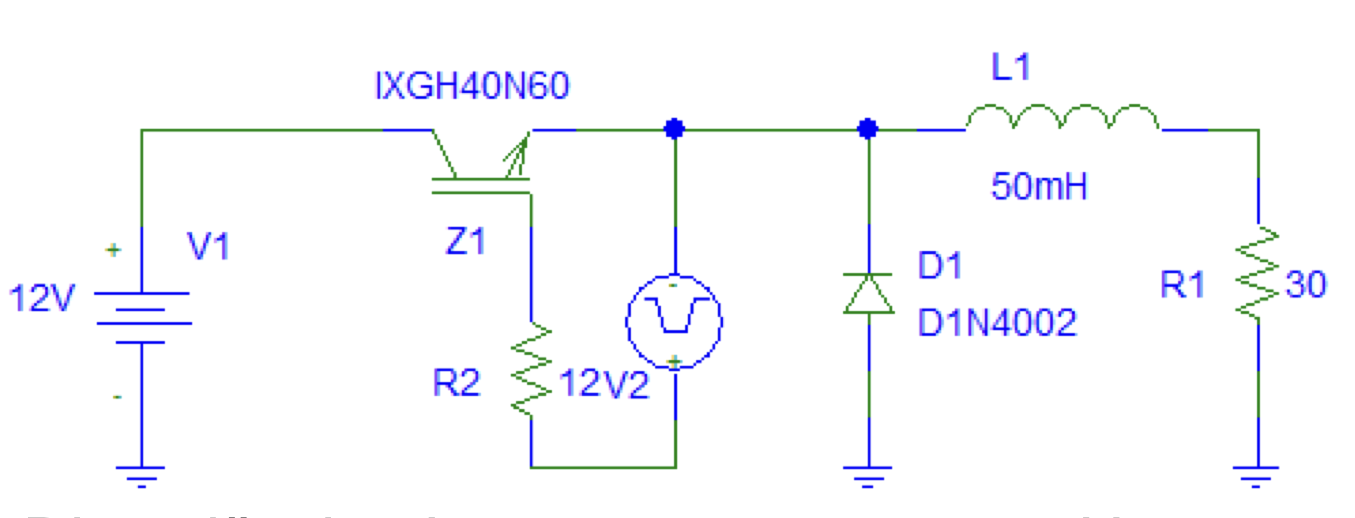
\includegraphics[width=0.85\linewidth]{images/Buckconverter.png}

\end{center}
Zeitverlauf Buck-Converter:
\begin{center}
    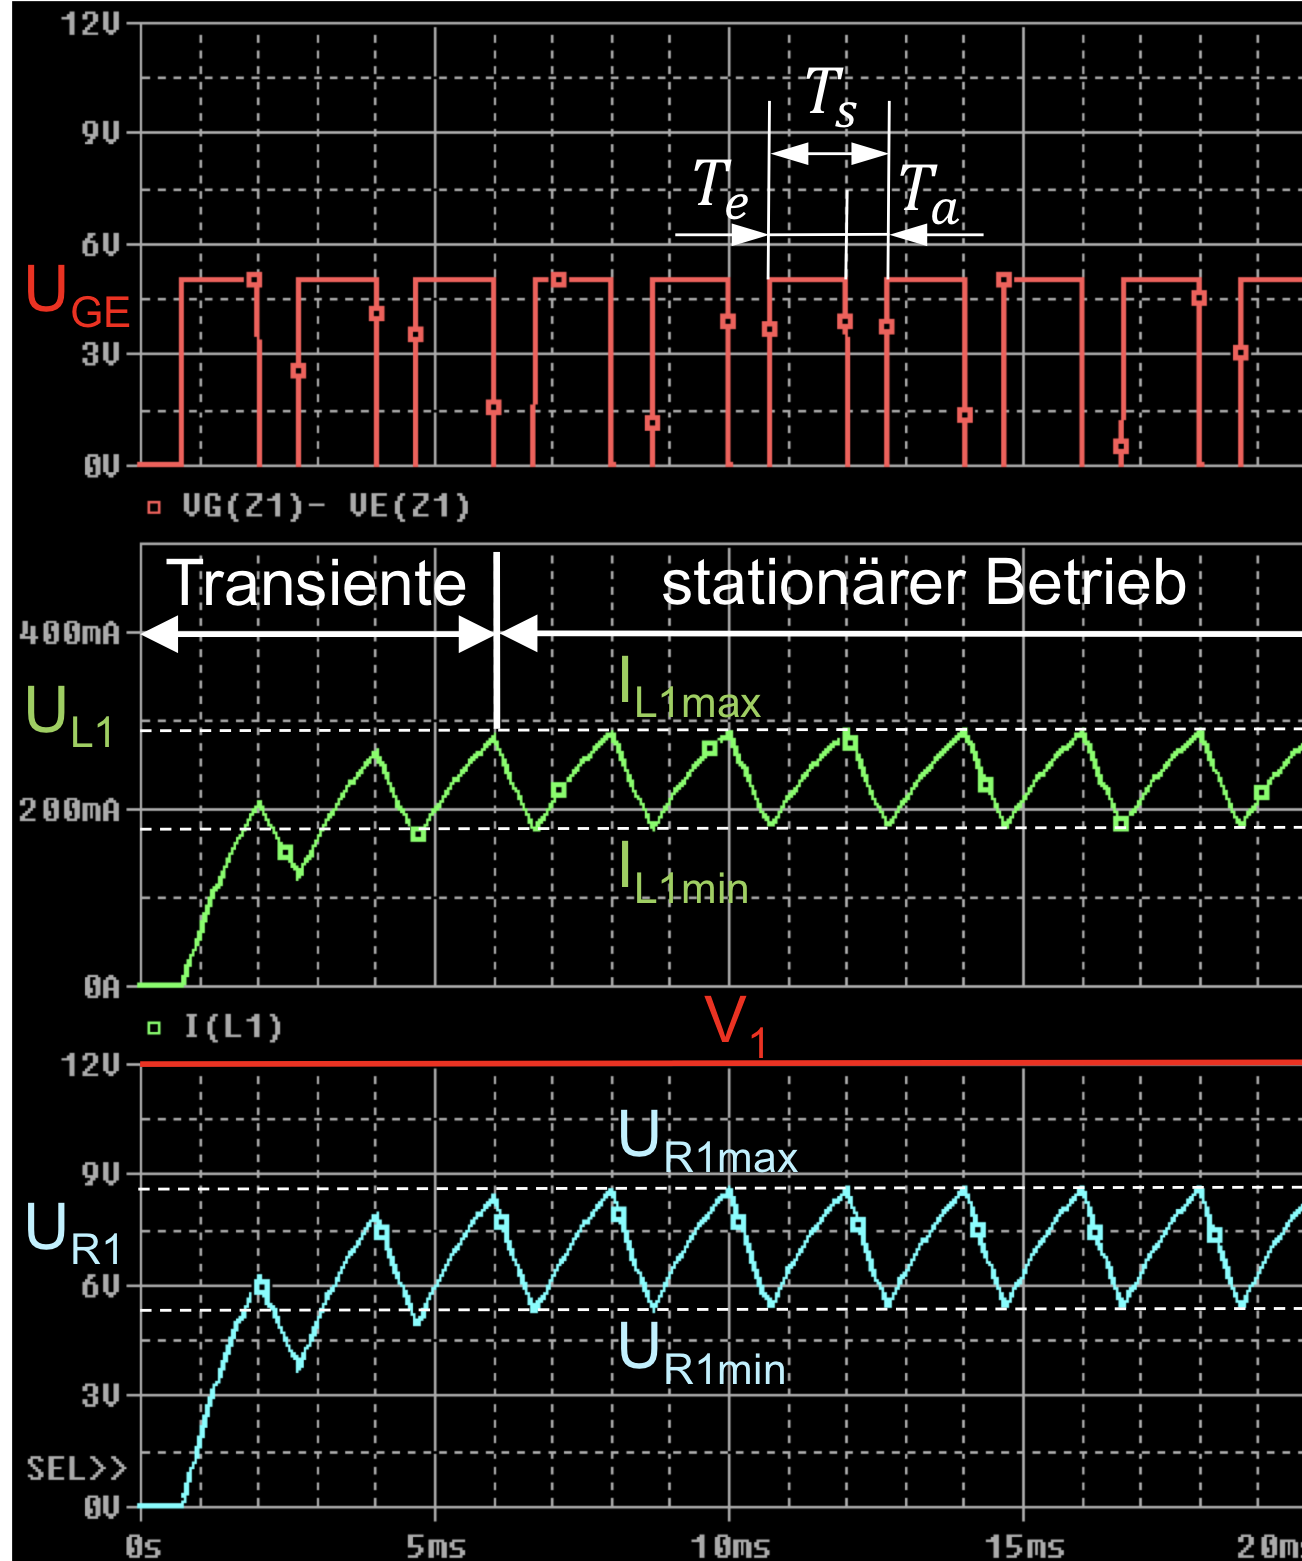
\includegraphics[width=0.85\linewidth]{images/Buckconverter_verlauf.png}
\end{center}
Ziel:
\[
u_2 < U_{DC}
\]

Mittelwert:
\[
\cbl{u_2 = d \, U_{DC}}
\]

Für $L < L_{\min}$ geht der Betrieb in den diskontinuierlichen Modus über.
Dann gelten die Mittelwertformeln nicht mehr exakt.

Eigenschaften:
\begin{itemize}
    \item Ausgangsspannung kleiner als Eingang
    \item Kontinuierlicher Ausgangsstrom
    \item Standardwandler in Netzteilen
\end{itemize}

% -------------------------------------------------
\subsection{Boost-Converter (Aufwärtssteller)}

% --- HIER: bestehende oder spätere Grafik Boost ---
\begin{center}
    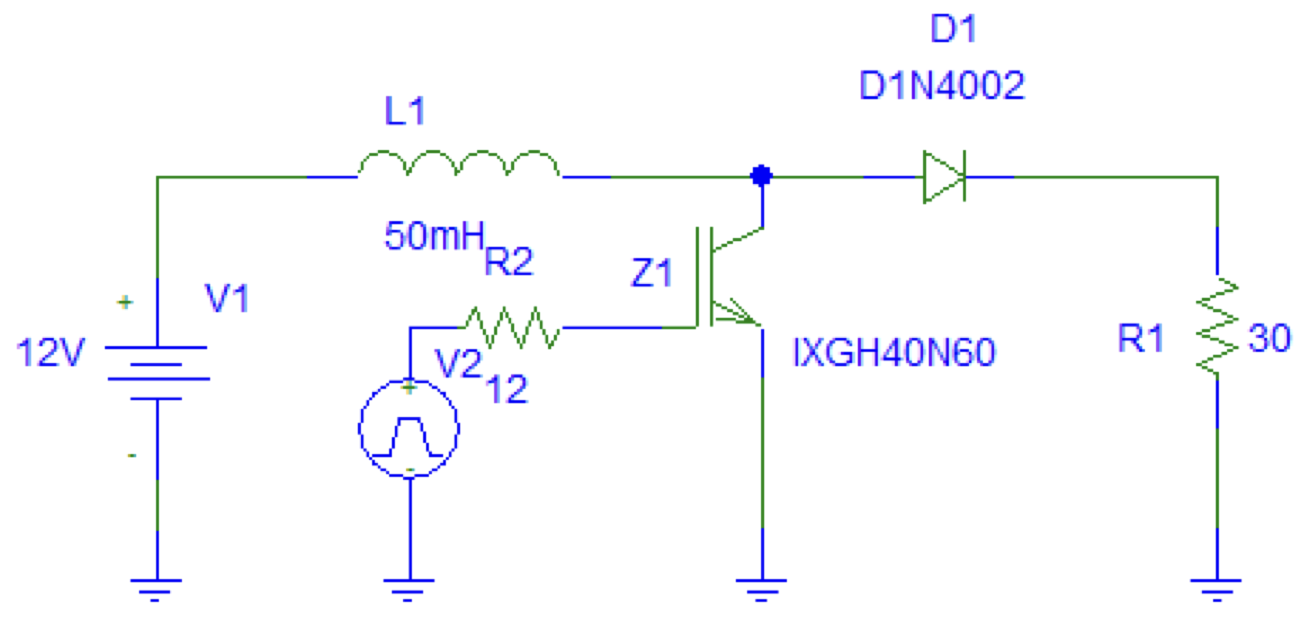
\includegraphics[width=0.85\linewidth]{images/Boostconv.png}
\end{center}
Zeitverlauf Boost-Converter:
\begin{center}
    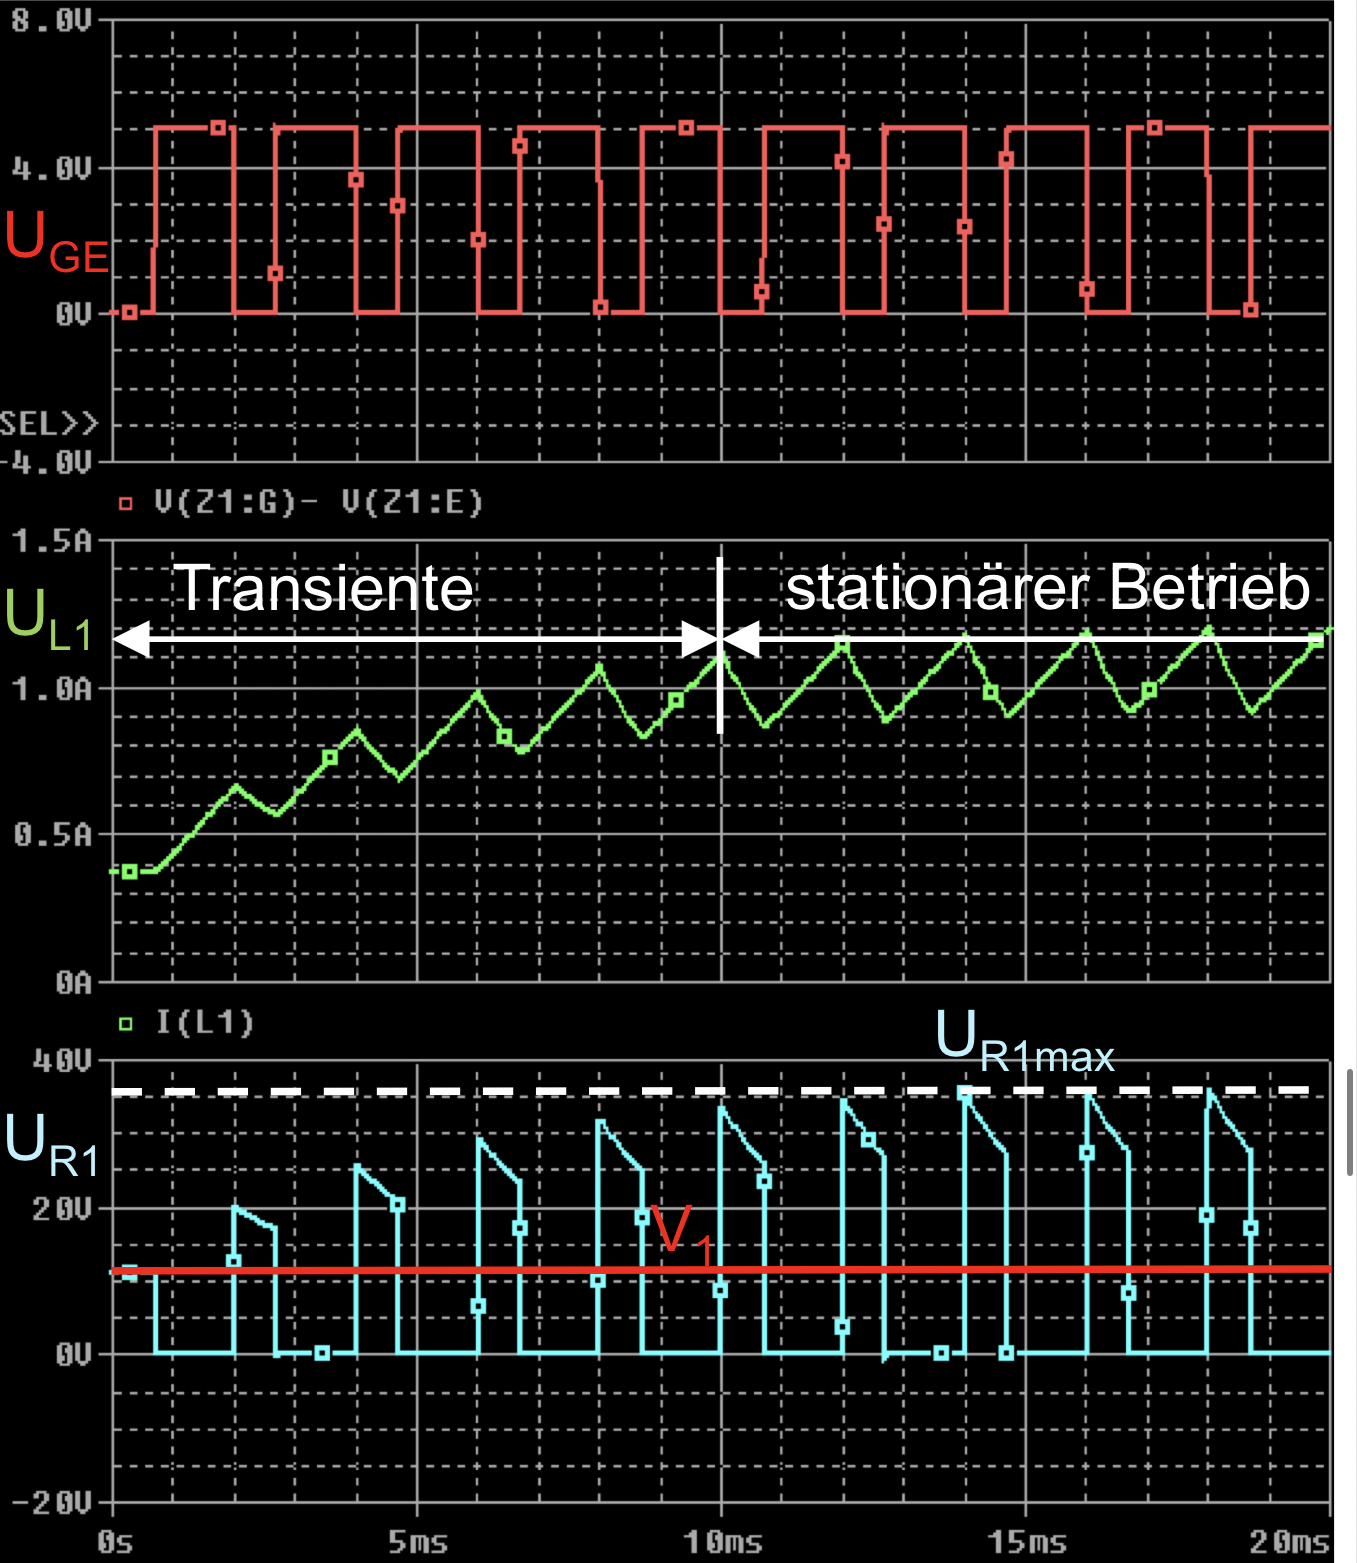
\includegraphics[width=0.85\linewidth]{images/Boostconv_verlauf.png}
\end{center}

Ziel:
\[
u_2 > U_{DC}
\]

Mittelwert:
\[
\cbl{u_2 = \frac{U_{DC}}{1-d}}
\]

Eigenschaften:
\begin{itemize}
    \item Ausgangsspannung grösser als Eingang
    \item Eingangsstrom gepulst
\end{itemize}

% -------------------------------------------------
\subsection{Buck-Boost-Converter}

% --- HIER: bestehende oder spätere Grafik Buck-Boost ---
\begin{center}
    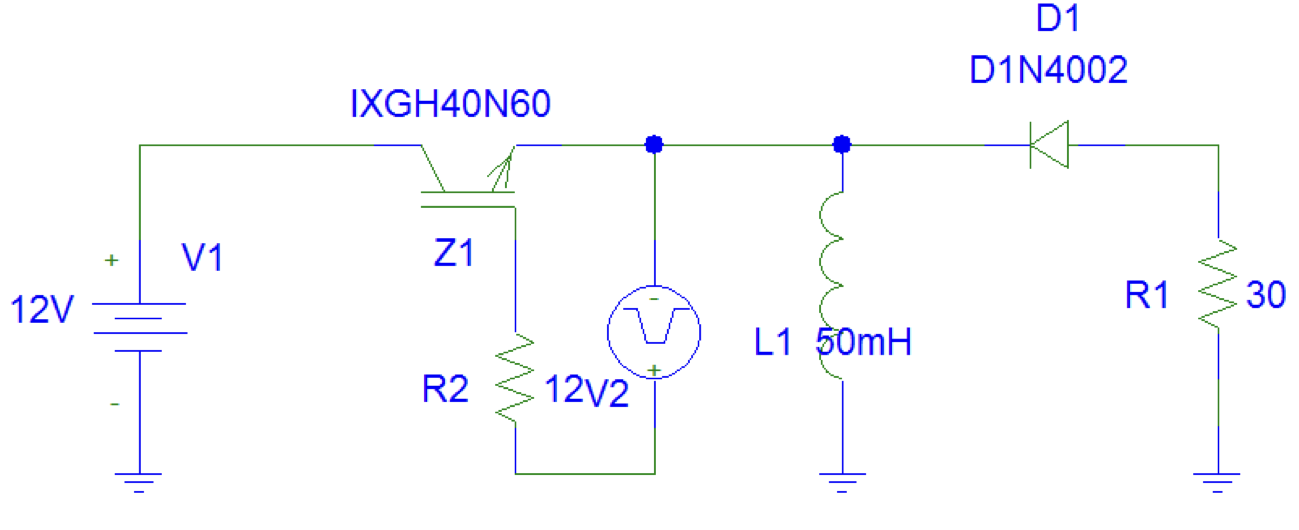
\includegraphics[width=0.85\linewidth]{images/Buckboostconv.png}
\end{center}
Zeitverlauf Buck-Boost-Converter:
\begin{center}
    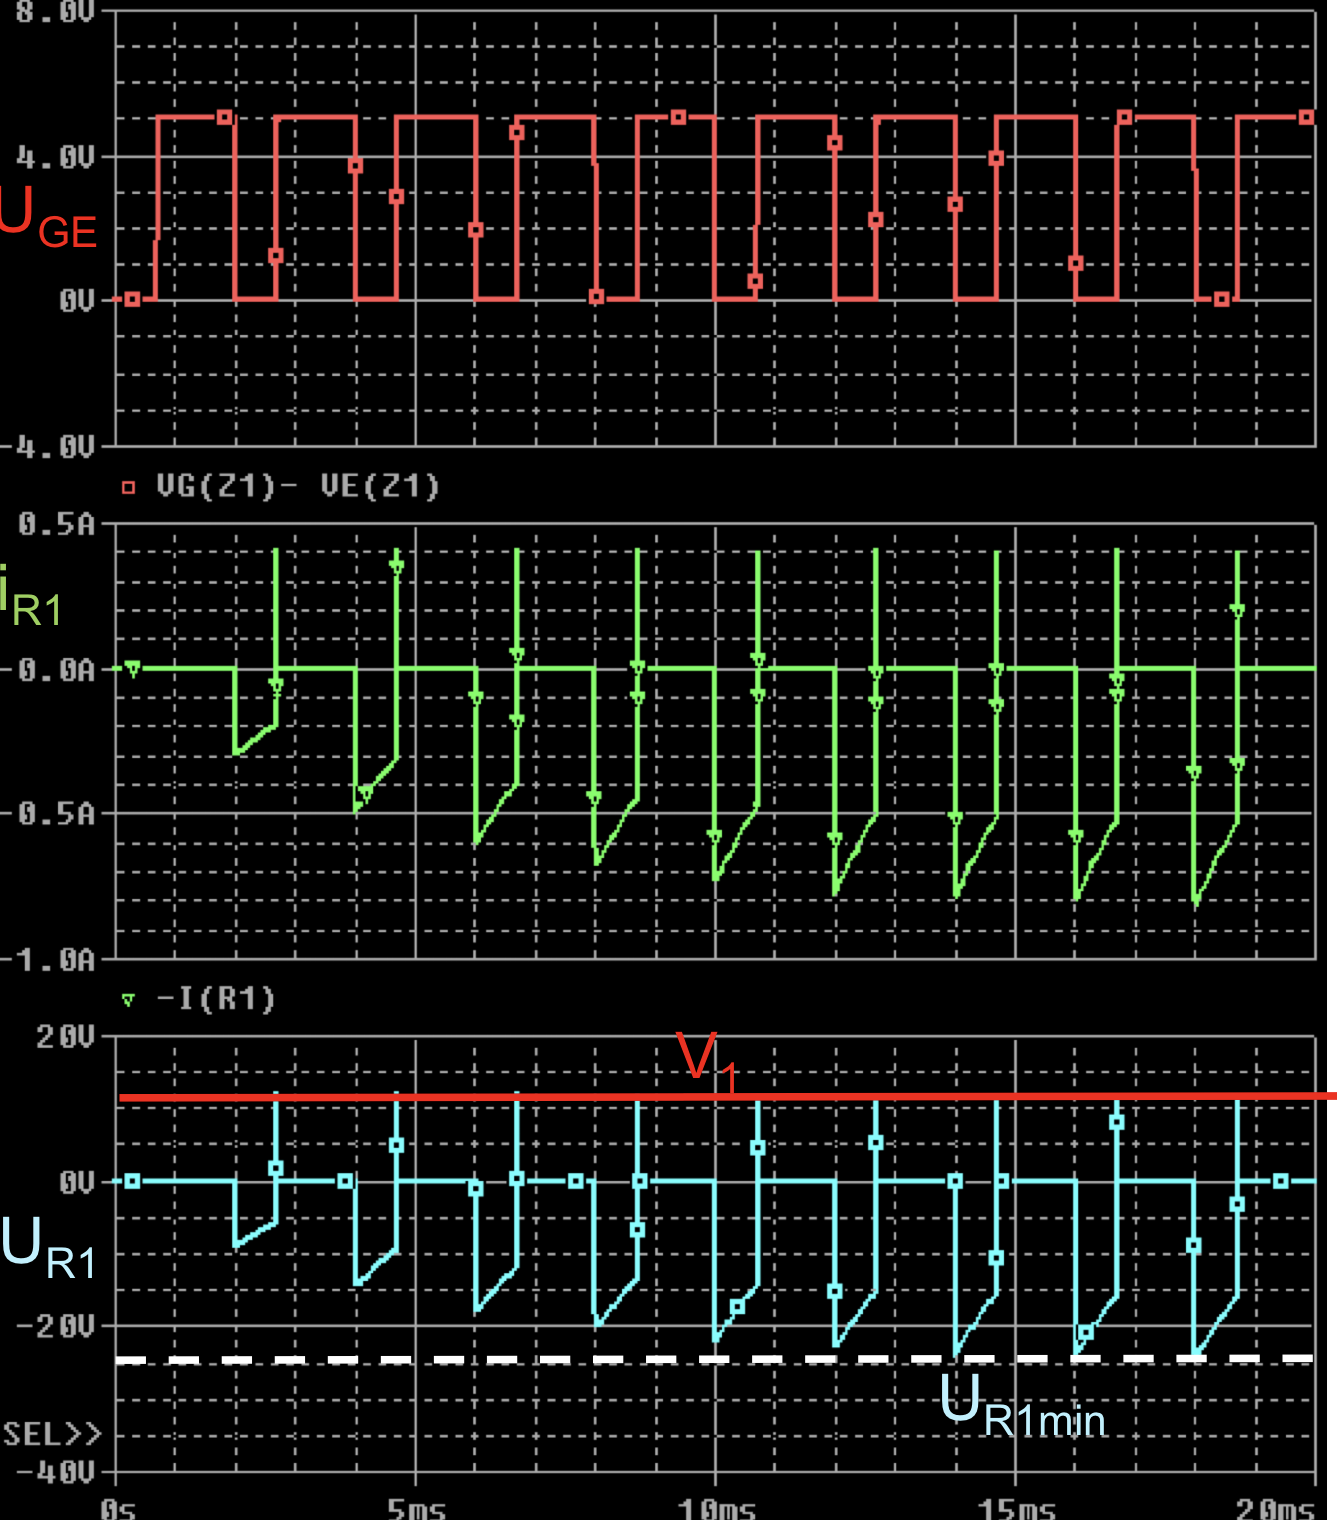
\includegraphics[width=0.85\linewidth]{images/Buckboostconv_verlauf.png}
\end{center}


Ziel:
\[
u_2 < 0 \quad \text{oder} \quad |u_2| > U_{DC}
\]

Mittelwert:
\[
\cbl{u_2 = -\frac{d}{1-d} U_{DC}}
\]
\paragraph{Stromrippel im Buck-Converter}
Im kontinuierlichen Betrieb gilt näherungsweise:
\[
\Delta i_L = \frac{(U_{DC} - u_2)}{L} \, d T_s
\]

Eigenschaften:
\begin{itemize}
    \item Polaritätsumkehr
    \item Spannung grösser oder kleiner als Eingang möglich
\end{itemize}

% -------------------------------------------------
\subsection{Vergleich der DC-DC-Wandler}

\begin{center}
\begin{tabular}{l|c|c|c}
 & Buck & Boost & Buck-Boost \\ \hline
$u_2/U_{DC}$ & $d$ & $\frac{1}{1-d}$ & $-\frac{d}{1-d}$ \\
Polarität & gleich & gleich & \cbl{invertiert} \\
$u_2<U_{DC}$ & \cbl{ja} & nein & ja \\
$u_2>U_{DC}$ & nein & \cbl{ja} & ja \\
\end{tabular}
\end{center}

\subsection{Abgrenzung zu klassischen Gleichstromstellern}

\begin{itemize}
    \item Klassischer Gleichstromsteller: direkte Pulsweitensteuerung der Last.
    \item DC-DC-Wandler: Energieübertragung über Induktivität mit Spannungsanpassung.
\end{itemize}

\crd{\textrightarrow\ Buck/Boost sind spezielle Gleichstromsteller mit Energiespeicher.}
